\chapter{Dynamic Taint Analysis}
Dynamic Taint Analysis (DTA), also called Data Flow Tracking (DFT), taint tracking or simply taint analysis allows for
the determination of the influence of a selected program state on other parts of the program state - e.g. tainting data
from the network and ensuring it is not changing the program counter in a control flow hijacking attack. Taint analysis
is normally implemented on top oof other instrumentation tools; in fact DTA instruments all of the instructions that
handle data in registers or memory. As for instrumentation this comes at a performance hit that is normally not
acceptable in production, thus DTA is relegated to offline use. DTA develops in three stages:
\begin{itemize}
    \item Defining taint sources;
    \item Defining taint sinks;
    \item Trackinkg taint propagation;
\end{itemize}



\section{Defining Taint Sources}
Taint sources are program locations where the data to be tracked is selected - e.g. syscalls, function entry points or
single instructions. Normally data are tainted by means of API calls, provided by the chosen DTA tool or library, that
take in input the register or the memory address of the tainted information.



\section{Defining Taint Sinks}
Taint sinks are program locations to be checked to see how they are influenced by tainted data; in order to do so the
instructions would need to be instrumented at taint sinks. DTA library allow defining taint sinks or checking if a
location is a taint sinks. Detecting taint data in sinks normally triggers a response or an alert.



\section{Tracking Taint Propagation}
In order to track the flow of tainted data all of the instruction handling that data must be instrumented in order to
establish how taint propagates from the input operands to the output operands. Taint propagation is bound to a taint
policy, detailed in the next section, that establishes the relationship between input and output operands.



\section{DTA Design Factors}
Complex DTA systems require tuning multiple factors that determine the trade off between performance and versatility of
the system; these are:
\begin{itemize}
    \item Taint Granularity;
    \item Number of Colors;
    \item Taint Policy;
\end{itemize}


\subsection{Taint Granularity}
Taint granularity is the unit of innformation by which the DTA system tracks taint - e.g. a bit-granular system keeps
track of whether each individual bit is in a register, whereas a byte-granular system tracks taint information only per
byte. Granularity can affect accuracy and performance of DTA - i.e. bit granularity is more accurate than byte
granularity, but has greater computational complexity and overhead.
\begin{figure}[!htbp]
    \begin{center}
        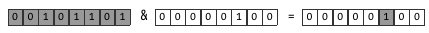
\includegraphics{./pics/bit-granular_taint.png}
        \label{bittaint}
        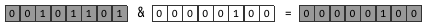
\includegraphics{./pics/byte-granular_taint.png}
        \label{bytetaint}
        \caption{Bit-granularity vs Byte-granularity}
    \end{center}
\end{figure}


\subsection{Taint Colors}
Sometimes the notion of tainted data is somewhat limited; if more information is needed, in order to understand where
the taint came from, data must be coloured. In a tainted/not tainted analysis a single bit is enough to understand the
taint of a piece of information, but if we want more colours we must use an additional bit for each one of them as to
allow for colours to be mixed - e.g. one byte can support eight different colors. Mixing colors is equivalent to the
bitwise OR; for example if a particular value is tainted by both the colors {\ttfamily 0x01} and {\ttfamily 0x02} then
the combined taint information will be {\ttfamily 0x03}.
